%% The first command in your LaTeX source must be the \documentclass command.
\documentclass[sigconf,authorversion]{acmart}
%% NOTE that a single column version may be required for
%% submission and peer review. This can be done by changing
%% the \doucmentclass[...]{acmart} in this template to
%% \documentclass[manuscript,screen,review]{acmart}

\begin{document}
\settopmatter{printacmref=false}
\setcopyright{none}
\renewcommand\footnotetextcopyrightpermission[1]{}
\pagestyle{plain}
\title{Progress Report for CSS 586 Project: \\
Music Generation Using Deep Learning}

%%
%% The "author" command and its associated commands are used to define
%% the authors and their affiliations.
%% Of note is the shared affiliation of the first two authors, and the
%% "authornote" and "authornotemark" commands
%% used to denote shared contribution to the research.

\author{Jack Phan}
\email{phan92@uw.edu}
\affiliation{%
  \institution{University of Washington}
  \city{Bothell}
  \state{WA}
  \country{USA}
}

\begin{abstract}

The original goal of the project is music transcription, which is the translation of audio data
to symbolic representation of musical notations. With further consideration, we decided to focus on 
a different problem to better align our work. The new objective is music generation using deep learning.
There are several methods that could be used to generate new music from a corpus of training data: MIDI, 
time-domain sound pressure data, frequency-domain representation of the sound pressure. Regardless of the 
data type, music generation involves the application of a sequence model such as recurrent neural network 
(RNN). The focus of my contribution is using a combination of time-domain and frequency-domain information. 
The current proges includes literature review, data exploration, learning about different representations 
of an audio signal. We are working on building a data pipeline and experimenting with various RNN models.
\end{abstract}

\keywords{deep learning, neural networks, music generation, RNN}

\maketitle

\section{Introduction}

Recurrent Neural Network (RNN) has shown its capability in recent years to model time-series sequences. 
Advanced version of RNN such as Gated Recurrent Unit (GRU) and Long Short-Term Memory (LSTM) have been 
successfully used for applications such as voice recognition, text to speech, and other applications 
that involve time-series data. RNN could also be used to generate novel sequences of texts or sounds.

A music recording is a digitized time-varying sequence of pressure displacement. Each point in the 
sequence represents the amplitude of the pressure strength at a moment in time. The sequence could 
also be converted to the frequency-domain representation, which describes its sound compoments in terms 
of amplitude and frequency. A popular representation of a sound segment is spectrogram. The goal of this 
project is generative modeling for short polyphonic music segments. We will build and train deep learning 
models using spectrogram as input, and generate novel music segments using these models.

\section{Related Work}

Musical generative modeling is an interesting area of research. Recent innovations in this domain involve
deep learning using a variety of modelling techniques. This section presents some of the recent works in
this domain.

Historically, the modeling of raw audio data is extremely challenging because a single second of audio recording
could contains up to 44,100 samples. Google DeepMind's WaveNet is one of the first models
that successfully learn from raw audio data \cite{oord_wavenet_2016}. It is designed using a technique called 
1D dialated causal convolution that allows an output to capture information from many inputs with a minimal
computational cost. WaveNet was designed for the primary purpose of generating speech which mimics any human voice.
Since the architecture can be used to model any raw audio signal, it was also used to generate music.
Although the outputs were far from being any masterpieces, the results show the possibility of generating musical
pieces from the raw audio data.

An alternatve representation of the time-series signal is the frequency-domain representation. Existing generative
models for audio have largely focused on the time-domain waveforms. In 2019, a generative model for audio in the
frequency domain called MelNet was introduced \cite{vasquez2019melnet}. MelNet models the spectrograms, which are
time-frequency representations of audio. The advantage of spectrograms is that they are compressed expressions of 
the time-domain signal. MelNet leverages this advantage to generate high-fidelity audio samples, which capture 
structures that are still challenging for time-domain models. 

\section{Planned Work}
The focus of this project is generating short musical pieces by modeling the spectrograms of input audio. The
following subsections describe our plan toward accomplishing this objective.

\subsection{Datasets}
We use a dataset called MusicNet published by University of Washington, the department of Computer Science 
\cite{thickstun2017learning}. This dataset is a collection of 330 freely-licensed classical music recordings 
captured under various studio and microphone conditions. The recordings are in .wav raw audio format and are
polyphonic, meaning that multiple musical notes could present at a single time point. Furthermore, the music is
performed by multiple instruments, which have unique sound signatures. 

\subsection{Data Processing}
Each training example is a raw sound fragment, which has a length of several seconds, taken from an audio recording.
We will transform the time-domain sample to the mel spectrogram representation. The mel scale is a logarithmic
transformation of a signal frequency. The idea of this transformation is to replicate the human perception of the 
difference between two sounds of different frequencies. For example, a person can easily tell the difference between 
100 Hz and 200 Hz, but cannot distinguish 1000 Hz and 1100 Hz. This transformation is done by splitting the sample
into overlapping windows, performing the Short Time Fourier Transformation on each window, converting the frequencies
to mel scale, and finally converting the amplitude to decibels. Librosa, a python package for music analysis, has
built-in functions for performing this tranformation. An example of a mel spectrogam is shown in Figure \ref{spectrogram}.

\begin{figure}[h]
  \centering
  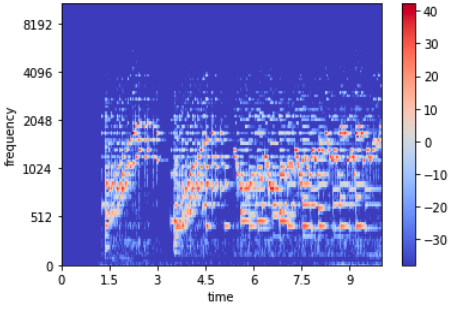
\includegraphics[width=\linewidth]{mel_spec.png}
  \caption{Mel spectrogram of a 10 second sound segment from the dataset. The color represents the magnitude in dB.}
  \label{spectrogram}
\end{figure}

\subsection{Model Building}
We will implement sequence models such as RNN, GRU, and LSTM to model the mel spectrogram and use these models to
generate novel spectrograms that could be converted back to audio.

\section{Progress}
Initially, a lot of time was spent on understanding different representations of the input data and on selecting a
viable representation that could be used to train a model. The key is that we can also reliably convert this
representation back to a sound wave. A number of representations are available: the raw waveform, the complex numbers,
the FFT of the waveform, the spectrogram, the mel spectrogram, and the mel frequency ceptral coefficients (MFCC). We decided
to use the mel spectrogram because it is a compressed version of the sound wave, which could be reliably convert back to 
audio. We also learned about the basics of sequence models such as RNN, GRU, and LSTM. Because the dataset is large and 
cannot be loaded into the memory at once, we are working on a data pipeline that processes the raw audio files and presents training examples 
one by one to a model. This pipeline will slice the input files into short audio fragments to be used as input. Then,
it will process the fragments as described in Section Data Processing. The resulting spectrograms will be save
to disk. The training code will load them into memory as needed to train the model.

\bibliographystyle{ACM-Reference-Format}
\bibliography{progress-jack}

\end{document}
\endinput
